\newpage
\section{Auswertung} % (fold)
\label{sec:auswertung}

Für die nachfolgende Auswertung wurden die Eigenschaften von Kupfer aus Tabelle \ref{Eigenschaften} verwendet.

\begin{table}{!h}
	\centering
	\caption[]{Eigenschaften von Kupfer \cite{kupfer1}\cite{kupfer2}.}
	\begin{tabular}{rrrrr}
		\toprule
		Masse/$\si{\gram}$ & Molmasse/$\si{\gram\per\mol}$ & $\rho \cdot 10^6/\si{\gram\per\meter^3}$ & $\Kappa \cdot 10^9/\si{\pascal}$ & $V_0 \cdot 10^{-6}/\si{\meter^3\per\mol}$\\
		\midrule
		342 & 63.546 & 8.92 & 7.11 & 140\\
		\bottomrule
	\end{tabular}
	\label{Eigenschaften}
\end{table}

\FloatBarrier
\subsection{Bestimmung von $C_\mathrm{V}$} % (fold)
\label{sub:bestimmung_von_c__mathrm}

\begin{table}[!h]
	\caption[]{Ergebnisse bei der Bestimmung von $C_\mathrm{V}$.}
	\centering
	\input{build/Cv.tex}
	\label{Cv}
\end{table}

\begin{table}[!h]
	\centering
	\caption[]{Werte zur Bestimmung von $C_\mathrm{P}$.}
	\input{build/data.tex}
	\label{Daten}
\end{table}

Die Ergebnisse zur Bestimmung von $C_\mathrm{V}$ sind in Tabelle \ref{Cv} dargestellt.
$C_\mathrm{P}$ konnte über
\begin{equation*}
	C_\mathrm{P} = \frac{M Q}{m \Delta T} = \frac{M t U I}{m \Delta T}
\end{equation*}
berechnet werden (\ref{Daten}).

Die Temperatur in Kelvin ist aus dem Widerstand mithilfe der Gleichung
\begin{equation*}
	T(R) = (0.0013658089 \pm 0.0000000011) \cdot R^2 + (2.293180 \pm 0.000019) \cdot R + (30.194 \pm 0.017)
\end{equation*}
berechnet worden, welche aus einer nicht-linearen Regression mithilfe der Methode der kleinsten Quadrate der Werte aus Tabelle \ref{Temperatur} gewonnen worden ist.

\begin{figure}[!h]
	\centering
	\caption[]{Temperatur in Abhängigkeit des Widerstandes \cite{V47}.}
	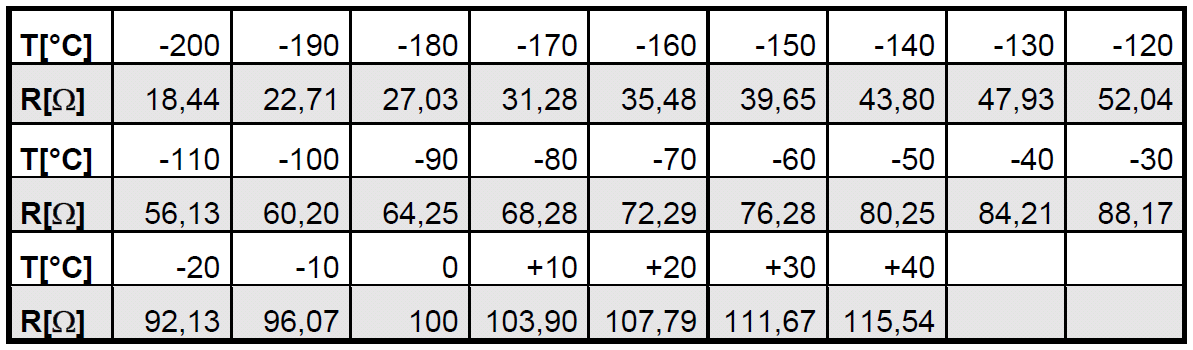
\includegraphics[width = 10cm]{img/temperatur.png}	
	\label{Temperatur}
\end{figure}

$C_\mathrm{V}$ lässt sich nun aus Gleichung \eqref{eqn:cp_cv} 
berechnen.
Dazu ist für die Temperatur der Mittelwert aus Anfangs- und Endwiderstand verwendet worden.
Der lineare Ausdehnungskoeffizient ist aus der Temperatur mithilfe der Gleichung
\begin{eqnarray*}
	\alpha(T) = 
	(4.412940810572491657\pm0.000000000000000004)10^{-17} &\cdot& T^5 +\\
	(-4.898243378402790\pm0.000000000000004)10^{-14} &\cdot& T^4 + \\
	(2.1799009653562\pm0.0000000000005)10^{-11} &\cdot& T^3 + \\
	(-4.93625747976\pm0.00000000013)10^{-9} &\cdot& T^2 + \\
	(5.958111139\pm0.000000009)10^{-7} &\cdot& T^1 + \\
	(-1.68738899\pm0.00000008)10^{-5} &&
\end{eqnarray*}
berechnet worden, welche aus einer nicht-linearen Regression mithilfe der Methode der kleinsten Quadrate der Werte aus Tabelle \ref{Alpha} gewonnen worden ist.

\begin{figure}[!h]
	\centering
	\caption[]{$\alpha$ in Abhängigkeit der Temperatur \cite{V47}.}
	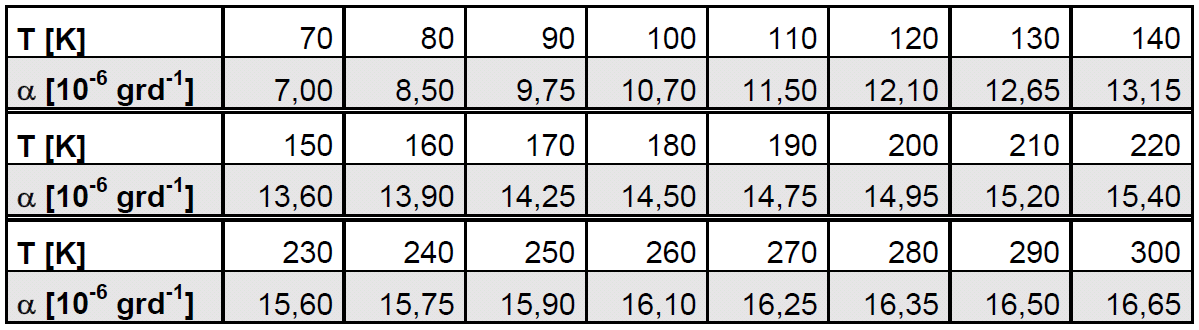
\includegraphics[width = 10cm]{img/alpha.png}	
	\label{Alpha}
\end{figure}

Die Ergebnisse sind Graphisch in Abbildung \ref{Cv_gra} dargestellt.
Zudem ist die Theoriekurve nach Gleichung \eqref{eqn:cv_debye} mit dem Theoriewert von $\Theta_D = \SI{345}{\kelvin}$ \cite{kupfer3}errechnet und der Abbildung hinzugefügt worden.

\begin{figure}
	\centering
	\includegraphics[width = 14cm]{build/Cv_Cv.pdf}
	\caption[]{Graphische Darstellung der Ergebnisse von $C_\mathrm{V}$ und der dazugehörigen Theoriekurve.}
	\label{Cv_gra}
\end{figure}

\subsection{Bestimmung der Debye Temperatur $\Theta_\mathrm{D}$} % (fold)
\label{sub:bestimmung_der_debye_temperatur_theta_mathrm}

\begin{table}[!h]
	\centering
	\caption[]{Ergebnisse der Berechnung der Debye-Temperatur.}
	\input{build/Theta.tex}
	\label{Theta_Debye}
\end{table}

\begin{figure}[!h]
	\centering
	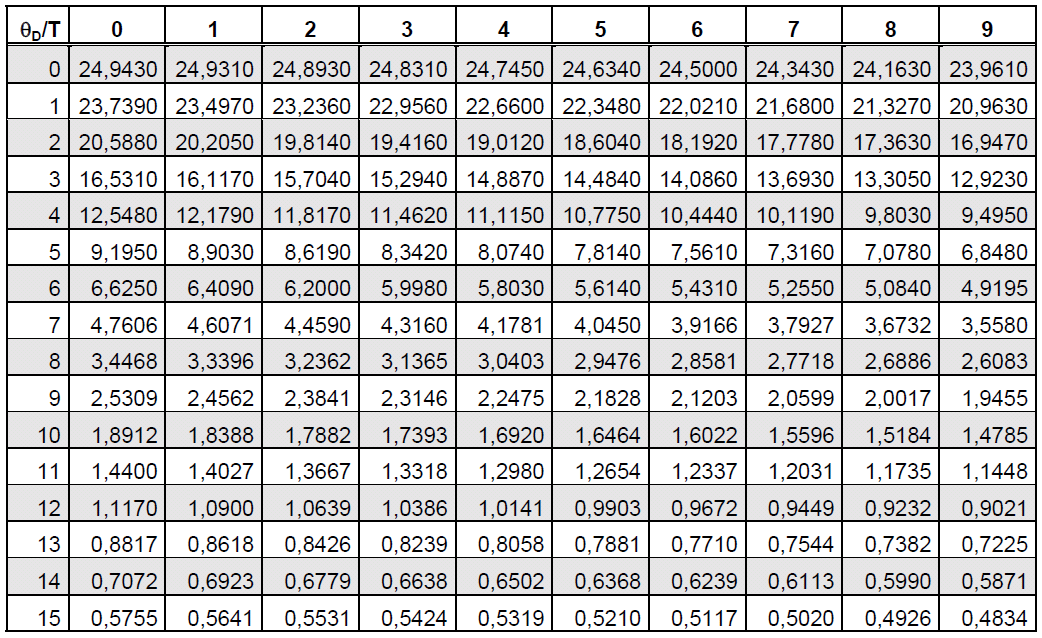
\includegraphics[width = 14cm]{img/theta.png}
	\caption[]{Werte der Universellen Debye-Funktion für $C_\mathrm{V}$ zur Bestimmung der Debye Temperatur $\Theta_\mathrm{D}$ \cite{V47}.}
	\label{Cv_global}
\end{figure}

Beim Vergleich der errechneten Werte von $C_\mathrm{V}$ bis zur Temperatur $T_\text{max} = \SI{170}{\kelvin}$ mit der Debye-Funktion aus Tabelle \ref{Cv_global} haben sich die in Tabelle \ref{Theta_Debye} dargestellten Werte für $\Theta_\text{D} / T$ ergeben.
Zudem hat ist es möglich durch Multiplikation mit der Temperatur auf den Wert für $\Theta_\text{D}$ zu schließen.

Durch Bilden des Mittelwertes der Debye Temperaturen konnte der Wert \input{build/theta_D.tex} errechnet werden.
\FloatBarrier
\subsection{Theoretische Berechnung von $\omega_\mathrm{D}$ und $\Theta_\mathrm{D}$} % (fold)
\label{sub:theoretische_berechnung_von_omega_mathrm}

Mithilfe der Gleichung \eqref{eqn:omega_debye}, den Geschwindigkeiten $v_\text{l}=\SI{4.7}{\kilo\meter\per\second}$ und $v_\text{l}=\SI{2.26}{\kilo\meter\per\second}$ und dem Zusammenhang
\begin{equation}
	N = N_\text{A} \frac{m}{M}
\end{equation}
ergiebt sich \input{omega_D_theo.tex}.
Daraus errechnet sich mithilfe der Gleichung
\begin{equation}
	\Theta_\text{D} = \frac{\hbar \omega_\text{D}}{\kb}
\end{equation}
zu \input{theta_D_theo.tex}.